\chapter[Green valley galaxies]{Identifying green valley galaxies}\label{ch:GV}

This work was done in collaboration with Jinfu Dai for his senior thesis 
``Exploring the green valley.''


\section{Introduction}

Large galaxy surveys \citep[like the Sloan Digital Sky Survey;][]{York00} 
revealed the structure of the color-magnitude diagram (CMD).  As seen in Fig. 
\ref{fig:ur_CMD}, the $u-r$ CMD is dominated by two major subgroups of galaxies: 
the red cloud and the blue sequence \citep{Strateva01, Baldry04}.  Most galaxies 
that reside in the red cloud appear to be older, elliptical galaxies that are no 
longer making stars (``red and dead'').  On the other hand, the blue sequence 
consists of mostly spiral and irregular galaxies which are actively forming stars.

% u-r CMD
\begin{figure}
    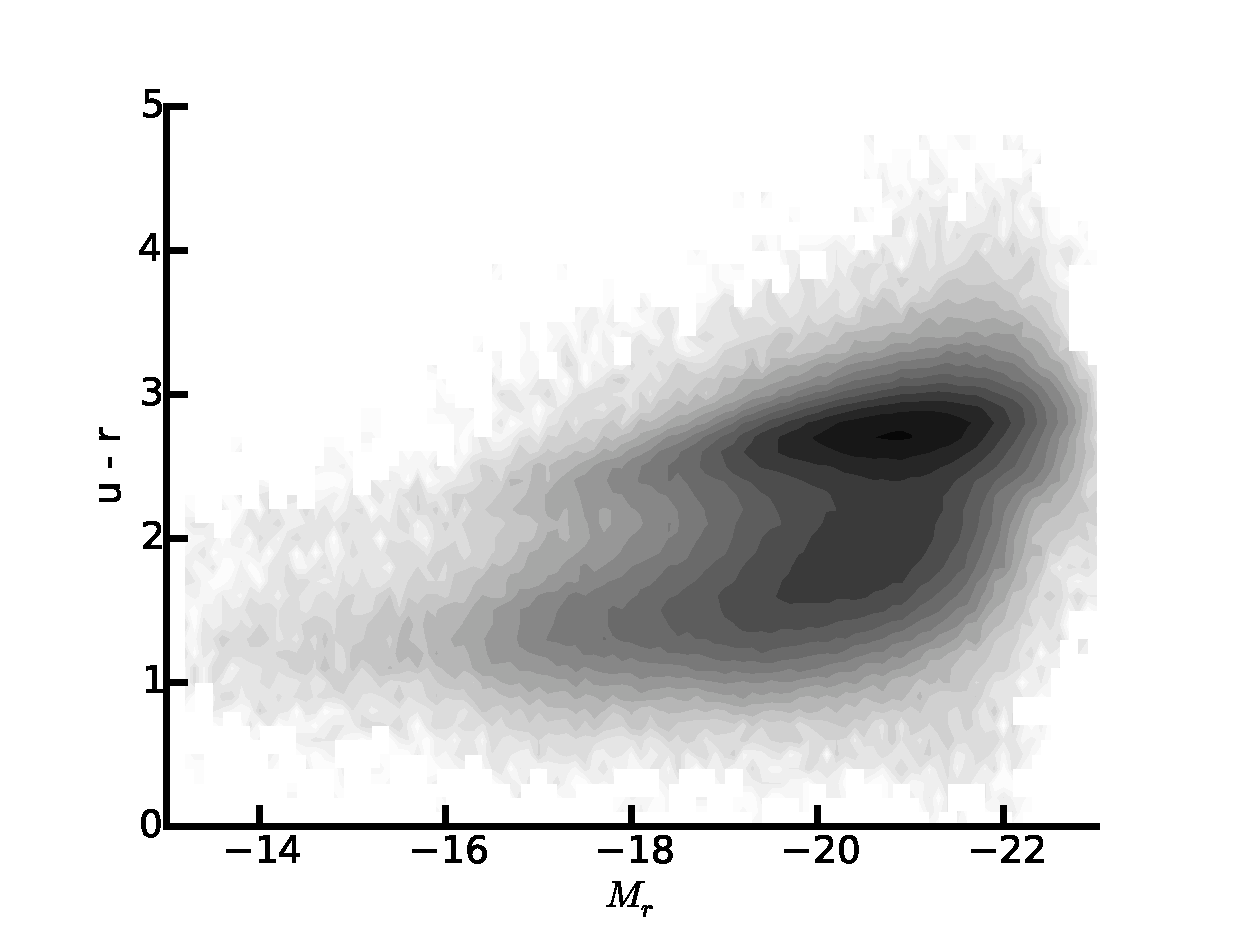
\includegraphics[width=0.49\textwidth]{Images/GV/ur_CMD_contour}
    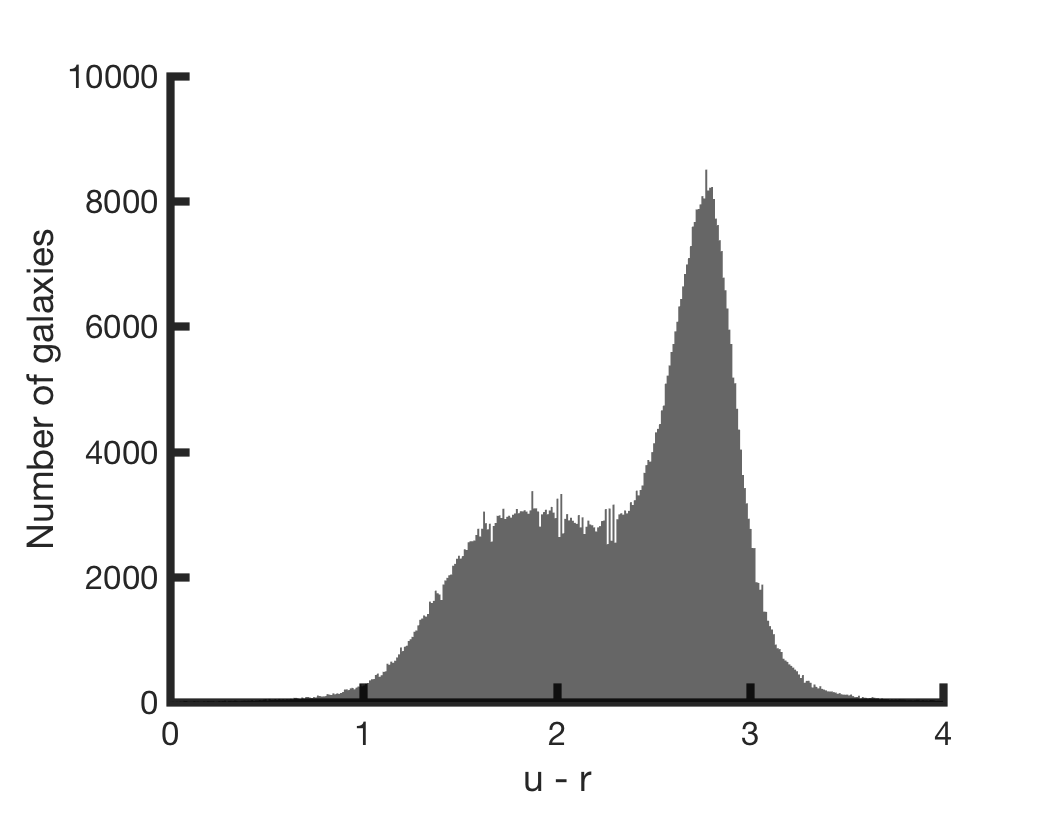
\includegraphics[width=0.49\textwidth]{Images/GV/ur_hist}
    \caption[Optical color-magnitude diagram and histogram of $u-r$ in SDSS]{The 
    optical color-magnitude diagram (left) and histogram of $u-r$ colors (right) 
    of galaxies in SDSS DR7.  There are two groups of galaxies, the populations 
    of which are well fit by the sum of two Gaussians.  They are aptly named the 
    ``red cloud'' and the ``blue sequence.''}
    \label{fig:ur_CMD}
\end{figure}

The enrichment of the interstellar medium (ISM) and circumgalactic medium (CGM) 
of a galaxy involves many complicated astrophysical processes, the interplay of 
which is not yet well understood.  A critical problem in galaxy formation is to 
understand how galaxies transition from the blue sequence to the red cloud of 
the optical color-magnitude diagram.  Star formation is thought to be quenching 
in galaxies moving through the green valley, but the relevant baryonic processes 
(gas cooling, feedback, etc.) are very complex and heavily interdependent.  
Investigating the star formation history and chemical evolution of galaxies in 
the green valley should provide clues as to the evolution of a galaxy through 
the color-magnitude diagram.

% VOGELEY THINKS THIS DESCRIPTION IS TOO SIMPLISTIC
%The current theory of galactic evolution describes a process in which a small 
%galaxy forms many stars in the beginning of its life.  As the galaxy merges with 
%others, it converts most of its hydrogen to heavier elements through 
%nucleosynthesis, and its rate of star formation slowly decreases.  The red, 
%elliptical galaxies we currently observe are hypothesized to be the remnants of 
%galaxies which have burned through the majority of their hydrogen; without fuel 
%for new stars, the galaxy's star formation rate eventually declines to a 
%negligible value.  As a result, most of the hot, massive blue stars have 
%expired, leaving behind smaller, cooler, more red stars.  These galaxies have a 
%redder color than their blue, star-forming predecessors.

% Feedback from AGN (strongly affects massive galaxies)
% Feedback from SN (dominates feedback in dwarfs)
% gas stripping interactions
% tidally-triggered star formation
There are a number of different astrophysical processes which simultaneously 
evolve a galaxy's stellar and gas content.  AGN feedback strongly affects 
massive galaxies, while dwarf galaxy feedback is dominated by supernovae.  Both 
AGN and supernovae can inject enough energy into a galaxy's ISM to prevent its 
cooling, thereby quenching star formation.  In addition to internal mechanisms, 
galaxies will often experience interactions in denser environmental regions.  
Depending on the properties of the galaxies involved (mass, speed, etc.), these 
interactions can either strip gas from the galaxy (removing a primary source of 
fuel for future star formation), or they can trigger a burst of star formation.

Our current theory of galactic evolution necessitates the existence of a 
transition period in a galaxy's lifetime, when the galaxy migrates from the 
star-forming blue sequence to the red cloud on the optical CMD.  However, the 
$u-r$ CMD is very well fit by the sum of only two Gaussians \citep{Strateva01, 
Baldry04}; an intermediate population is not present in the optical CMD.  Early 
explanations developed to reconcile this apparent discrepancy between theory and 
observation included a sudden transition from the blue sequence to the red 
cloud, often associated with some star-formation quenching mechanism.

Dubbed the ``green valley,'' it is thought that star formation 
is being quenched in the galaxies moving through the green valley 
\citep{Martin07}.  So far, results of studies done with these green valley 
galaxies have been inconclusive as to why or how this is occurs.


%%%%%%%%%%%%%%%%%%%%%%%%%%%%%%%%%%%%%%%%%%%%%%%%%%%%%%%%%%%%%%%%%%%%%%%%%%%%%%%%
%%%%%%%%%%%%%%%%%%%%%%%%%%%%%%%%%%%%%%%%%%%%%%%%%%%%%%%%%%%%%%%%%%%%%%%%%%%%%%%%


\section[Theory]{Calculating the color of a galaxy}

A galaxy's color is a logarithmic ratio of the ratio of the flux emitted by the 
galaxy in two different bands.  The stellar population of a galaxy will 
determine its color: redder galaxies contain much older, cooler stars, while the 
spectrum of a bluer galaxy is produced by light from much younger, hotter stars.  
While the KIAS-VAGC catalog (described below in Section \ref{sec:SDSS}) provides 
the $u-r$ color for all galaxies in SDSS, we make use of the Petrosian fluxes in 
the NSA (described in Section \ref{sec:GALEX}) to calculate the UV--optical 
color.  The NUV$-r$ color is calculated by
\begin{equation}
    \text{NUV}-r = -2.5\log \left( \frac{f_{NUV}}{f_r} \right)
\end{equation}
where $f_{NUV}$ is the Petrosian flux in the NUV-band of GALEX, and $f_r$ is the 
Petrosian flux in the $r$-band of SDSS.


%%%%%%%%%%%%%%%%%%%%%%%%%%%%%%%%%%%%%%%%%%%%%%%%%%%%%%%%%%%%%%%%%%%%%%%%%%%%%%%%
%%%%%%%%%%%%%%%%%%%%%%%%%%%%%%%%%%%%%%%%%%%%%%%%%%%%%%%%%%%%%%%%%%%%%%%%%%%%%%%%

\section[Data]{SDSS and GALEX data}

We use the photometric data from SDSS (optical) and GALEX (ultraviolet) as 
cross-matched in the NSA.

\subsection{Optical data --- SDSS}\label{sec:SDSS}
% Should we use NSA for abs. mag. instead? - yes, but not for the thesis

The SDSS Data Release 7 \citep[DR7;][]{Abazajian09} is a wide-field multi-band 
imaging and spectroscopic survey that uses drift scanning to map approximately 
one-quarter of the northern sky.  A dedicated 2.5-meter telescope at the Apache 
Point Observatory in New Mexico takes photometric data in the five-band SDSS 
system --- $u$, $g$, $r$, $i$, and $z$ \citep{Fukugita96,Gunn98}.  Galaxies with 
a Petrosian $r$-band apparent magnitude $m_r < 17.77$ are selected for 
spectroscopic analysis \citep{Lupton01,Strauss02}.  Gas-phase chemical 
abundances are calculated via the Direct $T_e$ method using emission-line fluxes 
measured by the MPA-JHU catalog\footnote{Available at 
\url{http://www.mpa-garching.mpg.de/SDSS/DR7}} and published in Douglass et al. 
(2017, in prep).  The large-scale environment of the galaxies is based on the 
void catalog compiled by \cite{Pan12}.  This void catalog is constructed from 
SDSS DR7 using the VoidFinder algorithm of \cite{Hoyle02}.  Galaxies which are 
located within the identified voids are labeled as void galaxies; those which do 
not reside in a void are designated as wall galaxies.  Because the minimum 
diameter of a void is defined as 10 \hMpc , the large-scale environment of 
galaxies within 5 \hMpc of the edge of the SDSS DR7 footprint cannot be 
described, so their environment is labeled as unknown.

% KIAS-VAGC (morphological classification)
The Korea Institute for Advanced Study Value-Added Galaxy Catalog 
\citep[KIAS-VAGC;][]{Choi10} contains galaxies from the SDSS DR7 main sky survey 
based on the New York University Value-Added Galaxy Catalog Data Release 7 
\citep[NYU-VAGC;][]{Blanton05}.  It provides a morphological class and type 
following the automated morphology classification scheme of \cite{Park05}, using 
the color $u-r$, color gradient $\Delta (g-r)$, and inverse concentration index.  
With these three quantities, galaxies are separated into one of three different 
morphological types: normal late type, normal early type, blue early type, and 
one of two different morphological classes: elliptical or lenticular and spiral 
or irregular.  For reference, typical star-forming spiral galaxies would be 
classified as a normal late type spiral or irregular galaxy, star-forming dwarf 
galaxies are usually normal late type spiral or irregular galaxies, and red 
elliptical galaxies are typically classified as normal early type elliptical or 
lenticular galaxies.  We use the absolute magnitudes as listed in the KIAS-VAGC.

\subsection{UV data --- GALEX}\label{sec:GALEX}
The Galaxy Evolution Explorer \citep[GALEX]{Martin05} is an orbiting space 
telescope conducting an extra-galactic ultraviolet all-sky survey.  The 
instrument allows imaging and spectroscopic observations in two ultraviolet 
bands: Far UV (FUV, 1350--1780\AA) and Near UV (NUV, 1770--2730\AA) 
\citep{Morrissey07}.  The NUV-$r$ colors used in this study are calculated from 
the azimuthally-averaged SDSS-style Petrosian fluxes provided in the NASA-Sloan 
Atlas version 0.1.2 \citep[NSA]{Blanton11}.


%%%%%%%%%%%%%%%%%%%%%%%%%%%%%%%%%%%%%%%%%%%%%%%%%%%%%%%%%%%%%%%%%%%%%%%%%%%%%%%%
%%%%%%%%%%%%%%%%%%%%%%%%%%%%%%%%%%%%%%%%%%%%%%%%%%%%%%%%%%%%%%%%%%%%%%%%%%%%%%%%


\section[Results]{Classification of galaxies in the color-magnitude diagram}

% CMD in NUV-r, showing where green valley galaxies live
\begin{figure}
    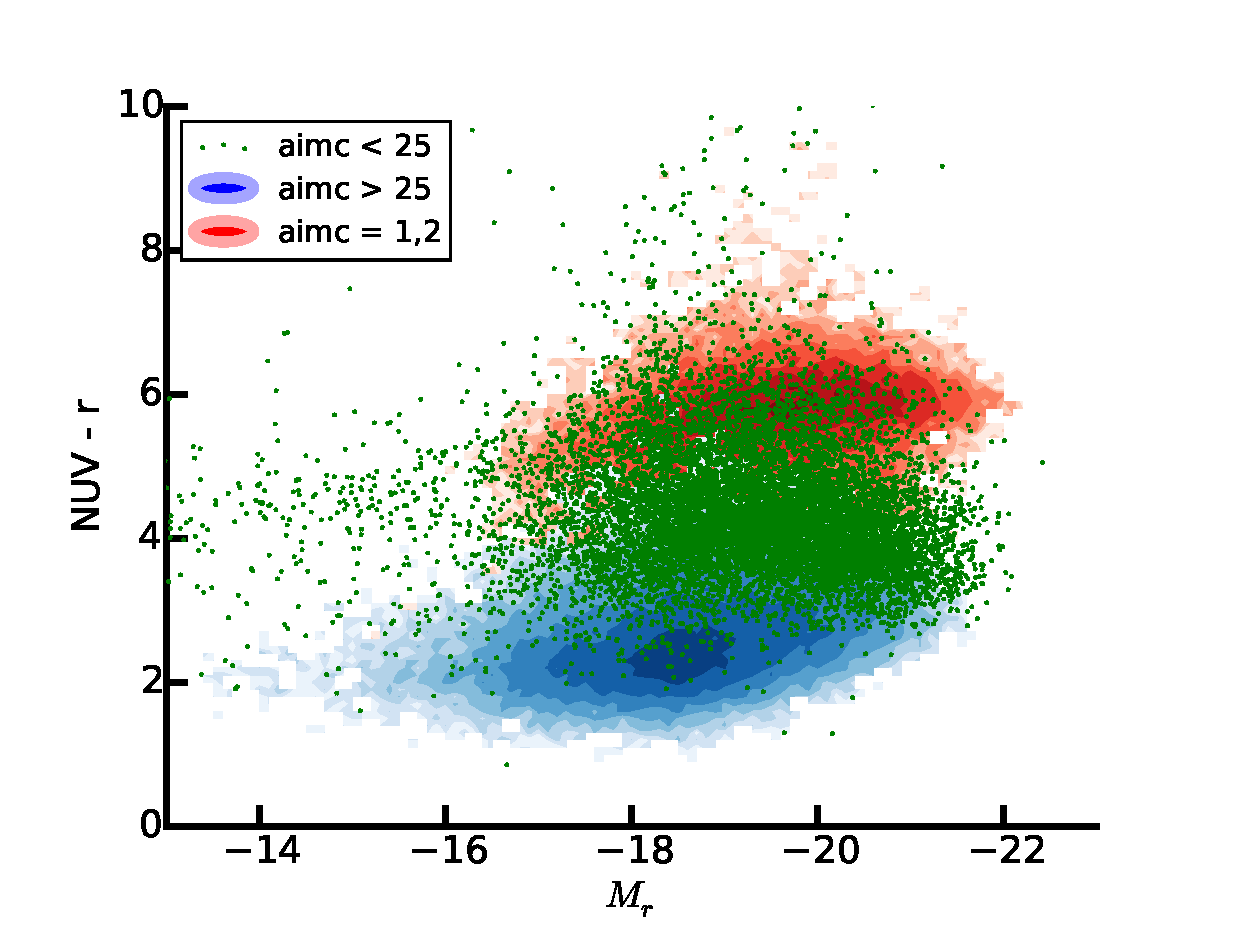
\includegraphics[width=0.65\textwidth]{Images/GV/NUVr_CMD_3pop_scatter}
    \caption[NUV-$r$ color-magnitude diagram of SDSS galaxies]{The NUV$-r$ 
    color-magnitude diagram of galaxies in SDSS DR7.  Those galaxies in the red 
    contours have morphological classifications of either normal early types 
    (aimc $=1$) or blue early types (aimc $=2$), as determined by the KIAS-VAGC.  
    The green points represent a subset of the normal late type galaxies (aimc 
    less than 25, excluding those with values of 1 or 2), and the blue contours 
    represents the remaining normal late type galaxies (aimc greater than 25).  
    It is clear that this morphological classification defines those galaxies 
    that are transitioning from the blue sequence to the red cloud.}
    \label{fig:NUVr_CMD}
\end{figure}

Combining the results of GALEX with the optical photometry of SDSS, we construct 
a NUV$-r$ CMD.  Probing light from even younger stars in the galaxies, GALEX is 
able to increase the separation of the blue sequence and red cloud populations 
of the optical CMD, revealing a third, smaller population of galaxies 
\citep{Wyder07}.

% Histogram of NUV-r, with all, red, blue, green galaxies (aimc values)
\begin{figure}
    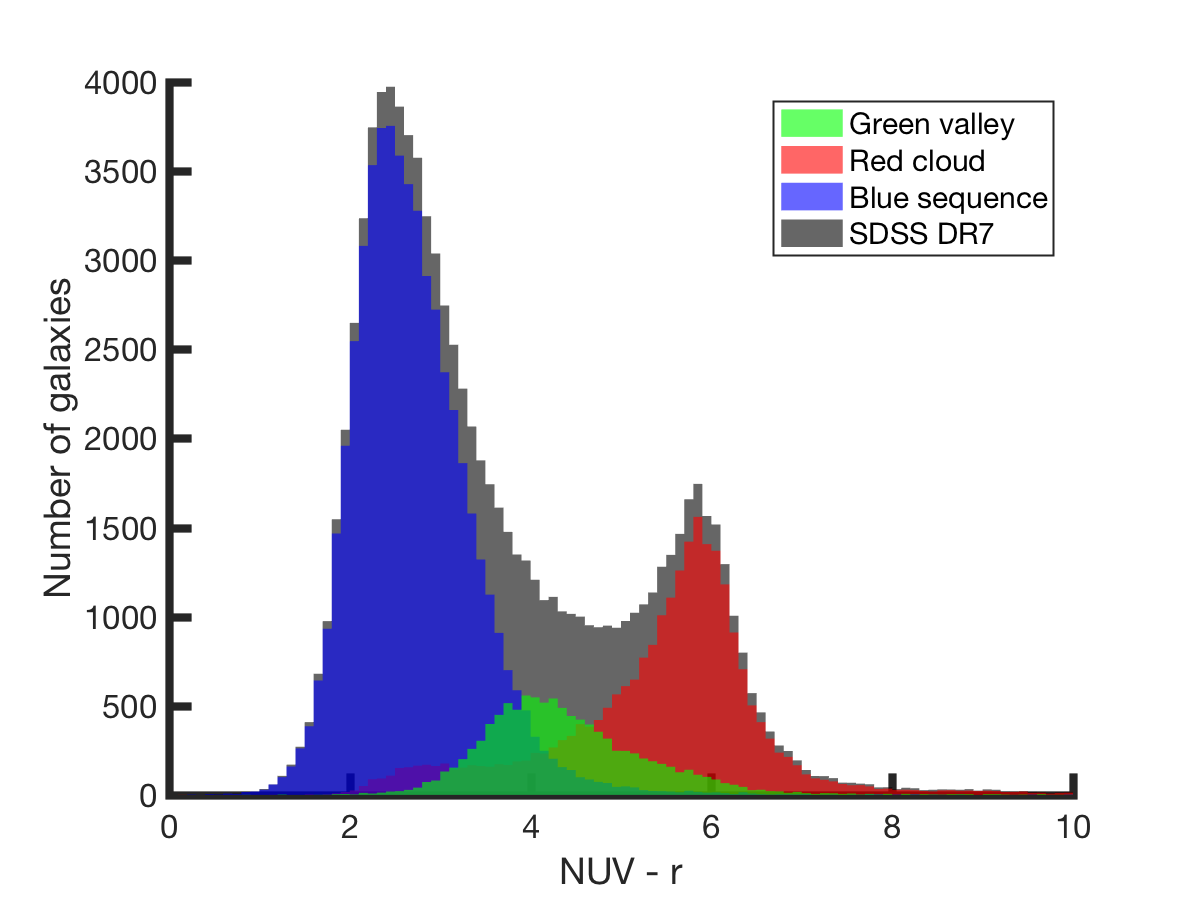
\includegraphics[width=0.65\textwidth]{Images/GV/NUVr_CMDclassifications}
    \caption[Distribution of NUV-$r$ of SDSS galaxies]{A histogram of the 
    NUV$-r$ color of those SDSS DR7 galaxies which are also detected in GALEX.  
    The red cloud, blue sequence, and green valley populations are separated by 
    the morphological types as defined by the KIAS-VAGC.  It is readily apparent 
    that the green valley galaxies exist in the space between the red cloud and 
    blue sequence.}
    \label{fig:NUVr_hist}
\end{figure}

This analysis reveals a population of galaxies that lie in the Green Valley on 
the NUV$-r$ color-magnitude diagram, identified independent of their location on 
the diagram.  Rather than being classified based on arbitrary limits placed on 
the NUV$-r$ values \citep[as done by][]{Schawinski14,Salim14a}, the galaxies can 
be easily separated into three distinct populations based on the galaxies' 
morphological types as calculated in the KIAS-VAGC; this can be seen in Fig. 
\ref{fig:NUVr_CMD}.  Here, we group together normal late type and blue early 
type galaxies, and we separate into two groups the normal late type galaxies 
based on their value of the morphological type quantity calculated in the 
KIAS-VAGC.  Defined by the $u-r$ color and the color gradient $\Delta (g-i)$, it 
is novel that an estimate of the morphological type of the galaxies is an 
adequate classification for the three populations of the NUV$-r$ CMD.  In 
addition, Fig. \ref{fig:NUVr_hist} shows a histogram of the galaxies which 
overlap in both GALEX and SDSS, separated by their morphological classification 
from the KIAS-VAGC.  It shows that the three populations are well fit by three 
Gaussians --- the new population in the middle is the transient galaxy 
population originally ``missing'' from the optical CMD.

% classical classification of morphology v. aimc (aimc appaers to be a good indication of the transition in galaxy evolution
The morphological classification that we use to isolate the green valley 
population is relatively unique in that it is analytic; morphological 
classification attempts are often completed in a more subjective manner 
\citep[such as the GalaxyZoo,][]{Lintott11}.  In particular, the 
morphological type provided in KIAS-VAGC is a combination of the color $u-r$ and 
the color gradient $\Delta (g-i)$.  Both these quantities are independent of the 
NUV$-r$ CMD, which is part of the novelty behind why this measure separates the 
galaxies into the three evolutionary stages of the CMD so well.


\subsection{Properties of the Green Valley Galaxies}

\subsubsection{Stellar mass}

\begin{figure}
    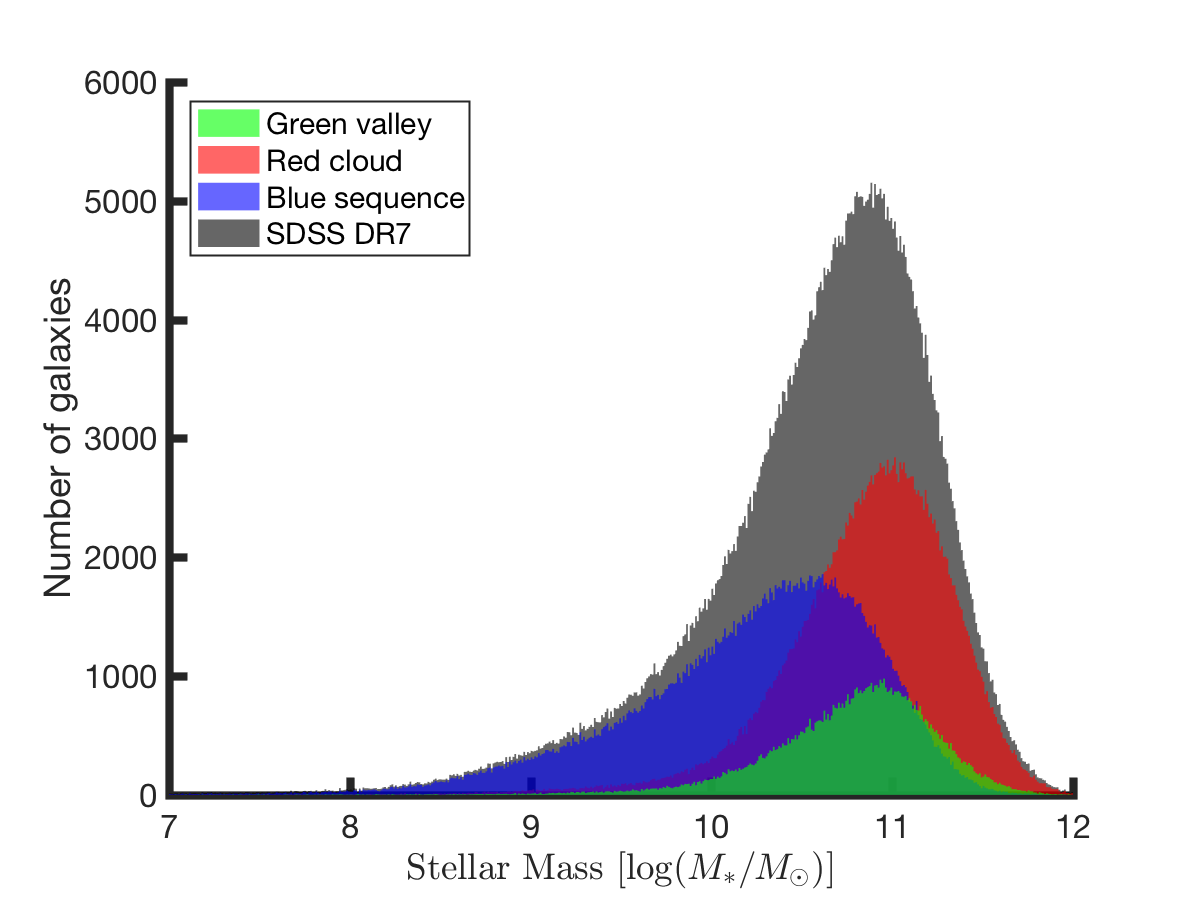
\includegraphics[width=0.65\textwidth]{Images/GV/Mstar_hist}
    \caption[Stellar mass distribution by morphological type]{The distribution 
    of stellar mass for all galaxies in SDSS DR7, separated by their 
    morphological type.  The galaxies in the green valley have stellar masses 
    comparable to those in the red cloud.  The stellar masses of those galaxies 
    in the blue sequence range from the lowest mass objects up through the 
    stellar masses of the green valley galaxies.}
    \label{fig:M_hist}
\end{figure}

If the green valley galaxies represent those galaxies transitioning between the 
blue sequence and red cloud, then their stellar masses should overlap the masses 
in both these populations.  The distribution of the stellar masses for the 
galaxies in SDSS DR7 is shown in Fig. \ref{fig:M_hist}.  We can see that the 
galaxies in the green valley have stellar masses comparable to those in the red 
cloud.  The stellar masses of those galaxies in the blue sequence range from the 
lowest mass objects up through the stellar masses of the green valley galaxies.  
The distribution of stellar masses of blue sequence galaxies should be much 
broader than the range of masses seen in the red cloud galaxies, since those in 
the blue sequence are slowly building up their stellar mass by forming stars 
from both their gas reservoirs and cool gas falling onto the galaxy.  Galaxies 
in the red cloud are fairly stagnant in their star formation, so the range of 
stellar masses of these galaxies will be more narrow than that of the blue 
sequence.  If the green valley galaxies are transitioning between the two 
populations due to a quenching of star formation or a sudden burst of star 
formation, then we would expect their mass range to cover the high-mass end of 
the blue sequence and most of the red cloud.  These expectations are met in Fig. 
\ref{fig:M_hist}.


\subsubsection{Star formation rates}

\begin{figure}
    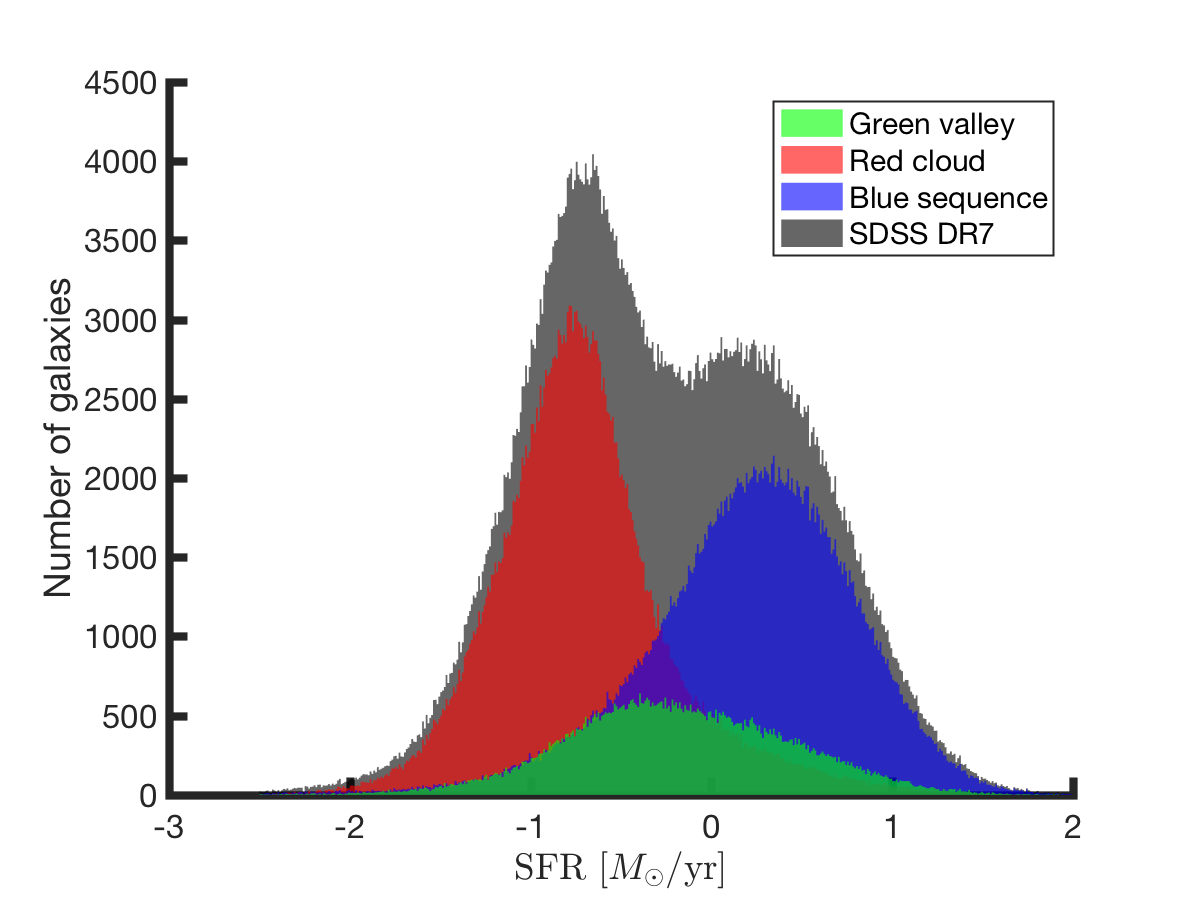
\includegraphics[width=0.49\textwidth]{Images/GV/SFR_hist}
    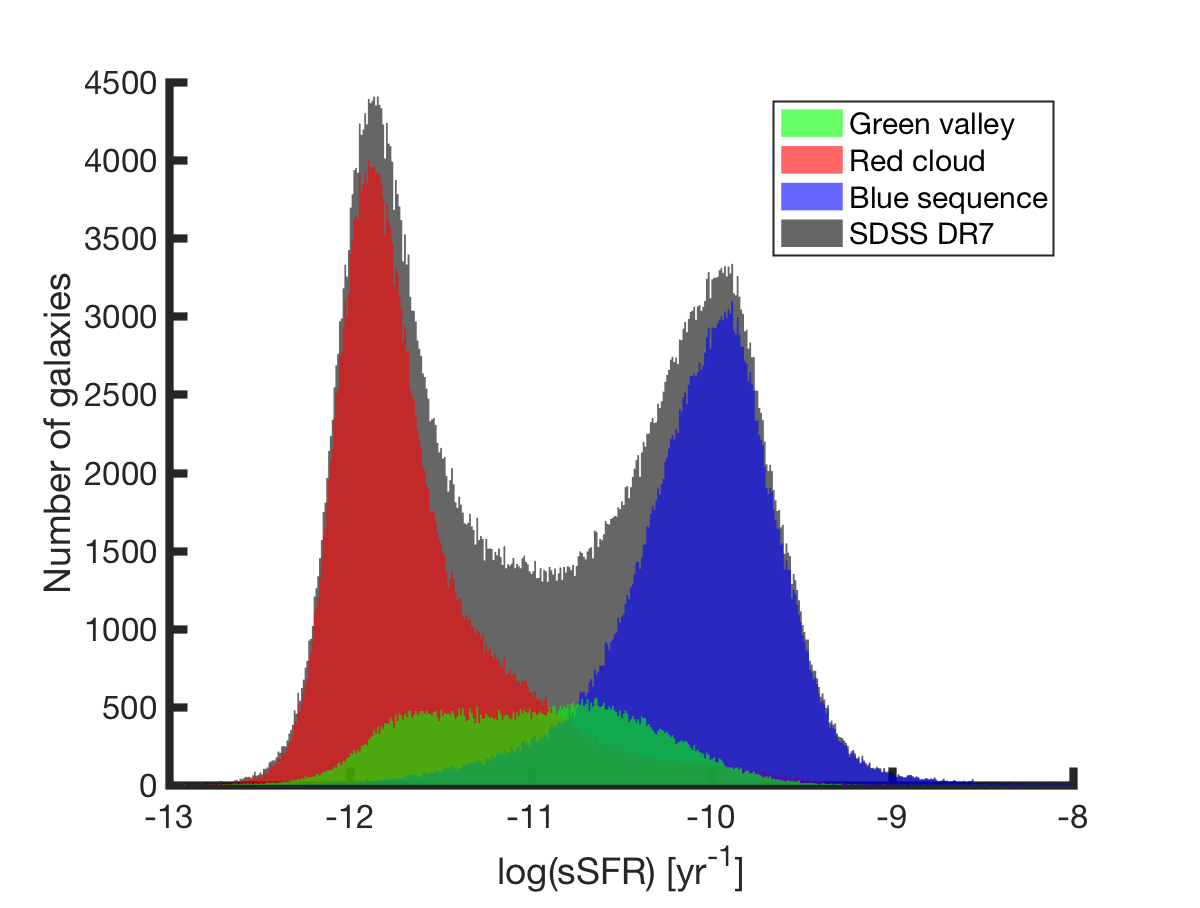
\includegraphics[width=0.49\textwidth]{Images/GV/sSFR_hist}
    \caption[(s)SFR distribution by morphological type]{The distribution of SFR 
    (left panel) and sSFR (right panel) for all galaxies in SDSS DR7, separated 
    by their morphological type.  The green valley galaxies occupy the 
    intermediate SFRs, while galaxies in the red cloud have low SFRs and 
    galaxies in the blue sequence have higher SFRs.  The same ranges exist for 
    the sSFRs, although the green valley galaxies extend well into the range of 
    sSFRs occupied by the galaxies in the red cloud.}
    \label{fig:SFR_hist}
\end{figure}

If green valley galaxies are transitioning between the blue sequence and red 
cloud, then they should have intermediate (s)SFRs.  The distribution of SFR and 
sSFR for the galaxies in SDSS DR7 are shown in Fig. \ref{fig:SFR_hist}, with the 
galaxies separated by their morphological types.  We see that the distribution 
of SFRs for galaxies in the green valley peaks around 
$\log(\text{SFR}) \sim -0.5$, in between the ranges occupied by the red cloud 
and blue sequence galaxies.  A similar distribution is shown for the sSFRs, 
although the green valley galaxies extend well into the range of sSFRs occupied 
by the galaxies in the red cloud.  \cite{Salim14a} finds transitional galaxies 
(those in the green valley) to have lower sSFRs than galaxies in the blue 
sequence, specifically $-11.8 < \log(\text{sSFR}) < -10.8$.  While our results 
do indicate that green valley galaxies have lower sSFRs than those in the blue 
sequence, we find that their range of sSFR is almost double the width of that 
described in \cite{Salim14a}.  The green valley galaxies have a sSFR within the 
range $-12 \lesssim \log(\text{sSFR}) \lesssim -10$.


\subsubsection{Gas-phase chemical abundances}

% Histogram of metallicity for red, blue, green galaxies
\begin{figure}
    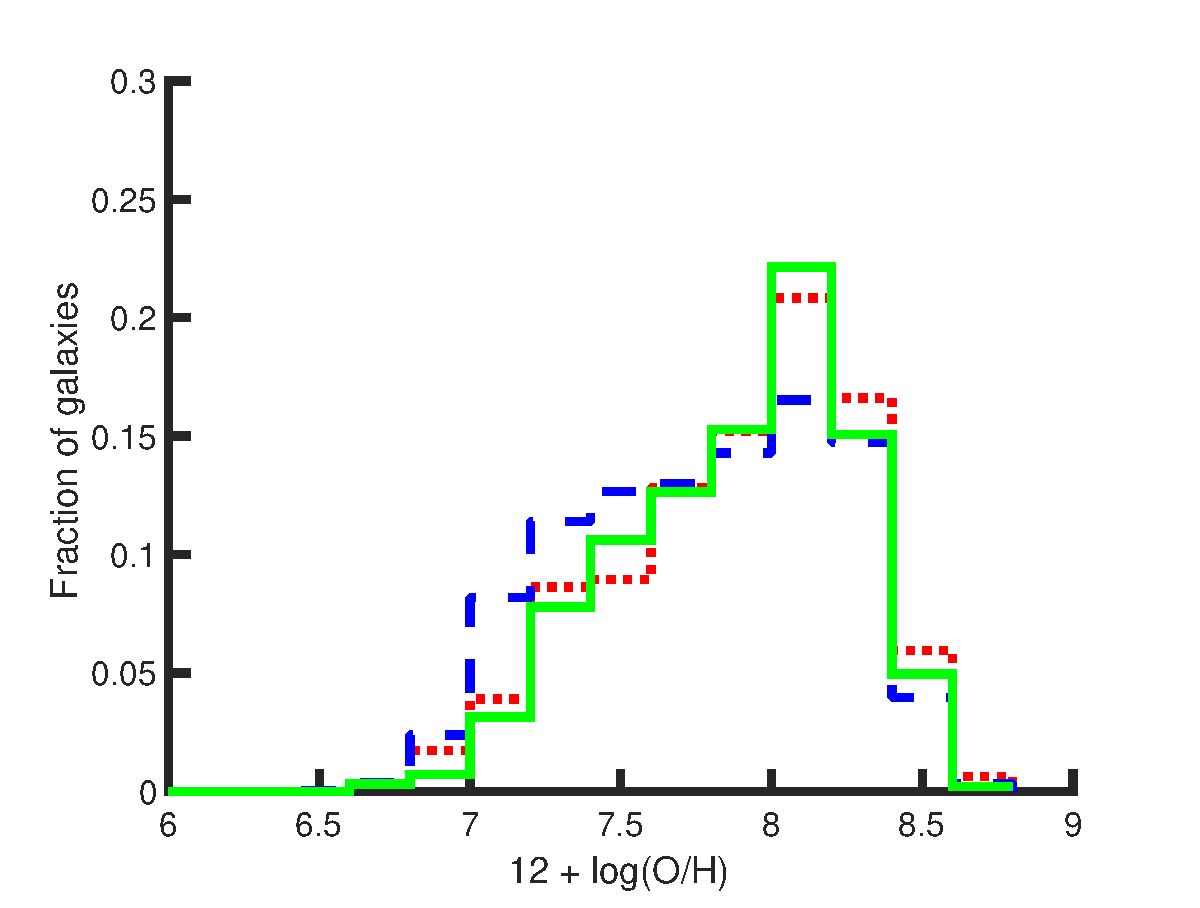
\includegraphics[width=0.49\textwidth]{Images/GV/Z12logOH_I06relations_t3}
    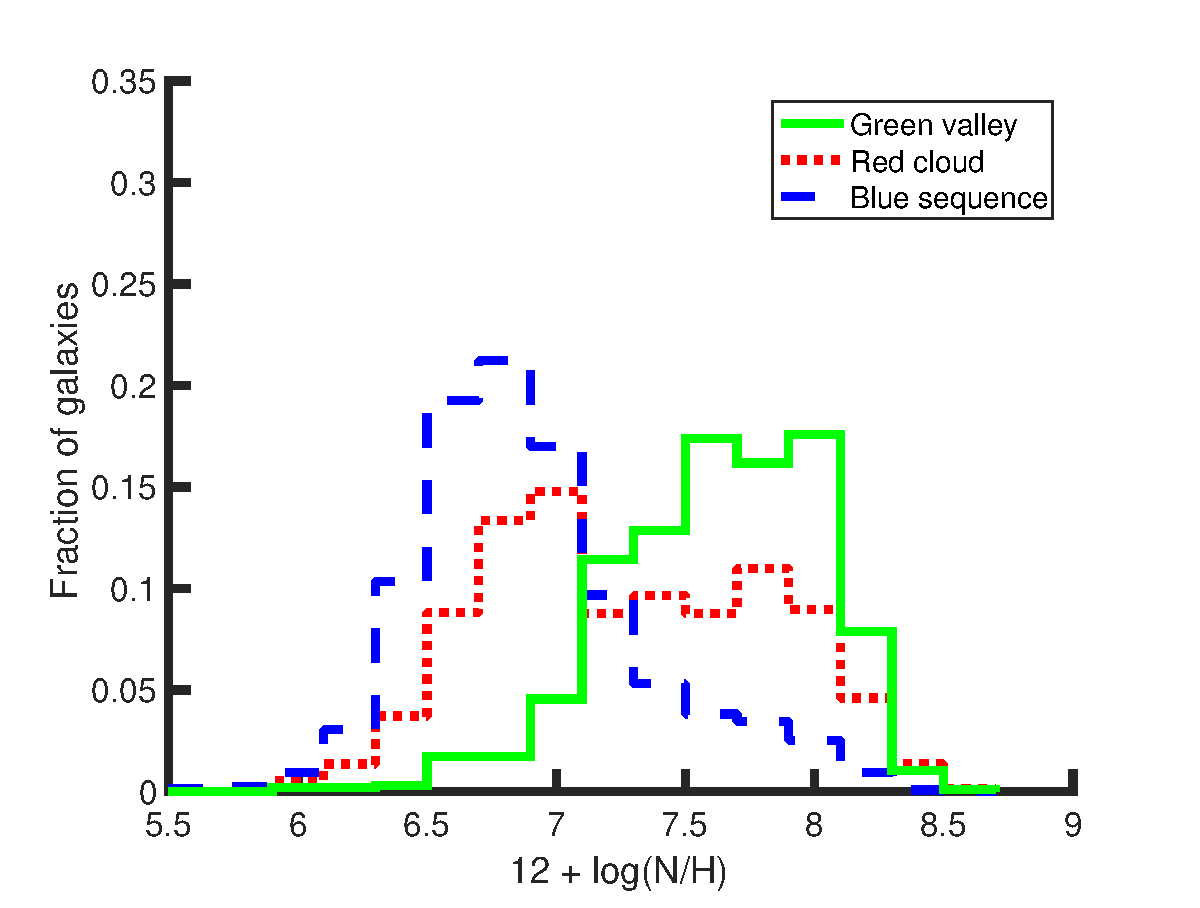
\includegraphics[width=0.49\textwidth]{Images/GV/N12logNH_I06relations_t3}
    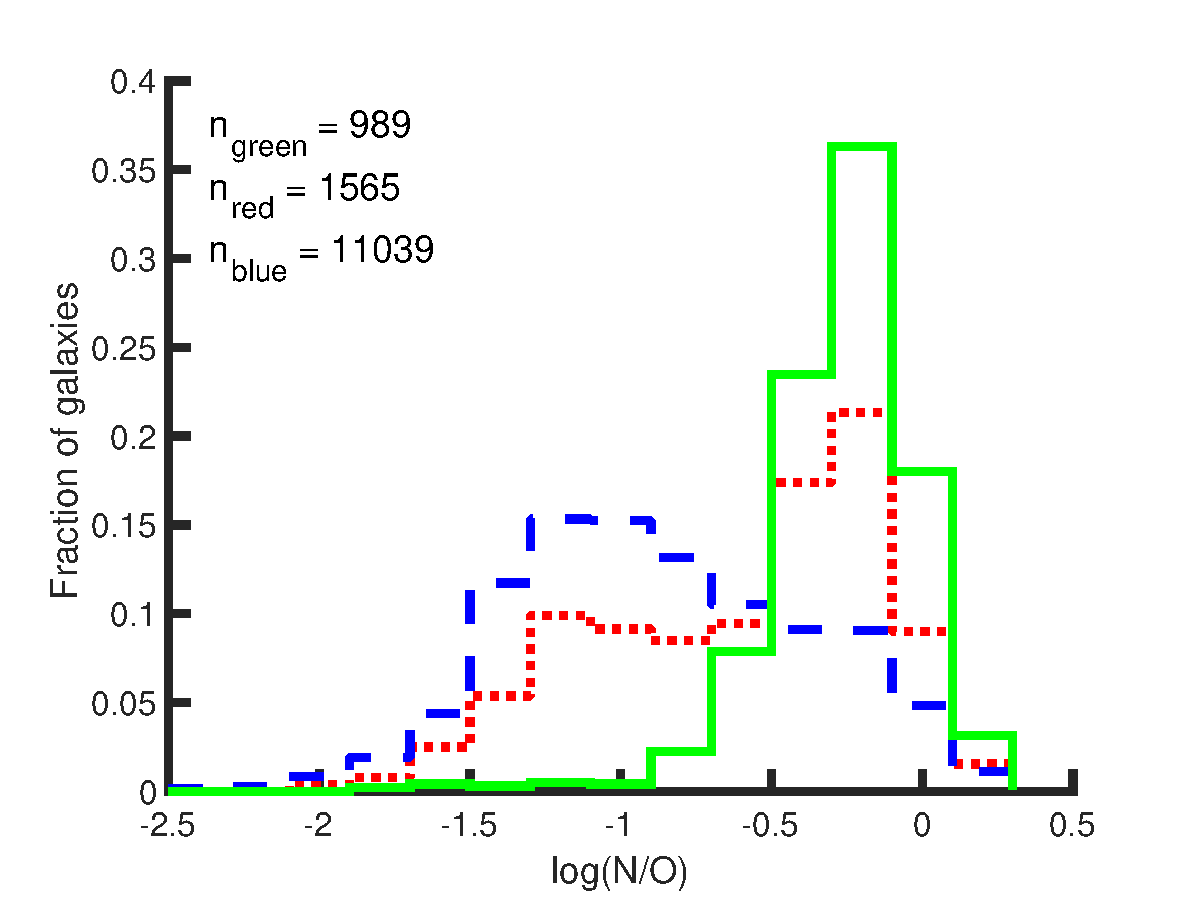
\includegraphics[width=0.49\textwidth]{Images/GV/logNO_I06relations_t3}
    \caption[Distribution of gas-phase chemical abundances in cross-matched SDSS 
    DR7 -- GALEX galaxies]{Histograms of the oxygen abundance (top left), 
    nitrogen abundance (top right), and N/O ratio (bottom center) of the 
    cross-matched SDSS DR7 -- GALEX galaxies, separated into their locations on 
    the NUV$-r$ color-magnitude diagram according to the morphological type 
    listed in the KIAS-VAGC.  It is readily apparent that the green valley 
    galaxies have higher nitrogen abundances than those in the blue sequence 
    (and some of the red cloud).  This, therefore, corresponds to them having 
    high N/O ratios.}
    \label{fig:Z_hist}
\end{figure}

Estimates of the gas-phase chemical abundances of galaxies probe their 
integrated star formation histories, which can provide insight into the 
enrichment of the ISM and CGM.  A few of the galaxies for which Douglass et al. 
(2017, in prep) are able to estimate metallicities reside in the green valley.  
When compared with the metallicities of galaxies in the blue sequence and red 
cloud, Fig. \ref{fig:Z_hist} shows that the green valley galaxies have higher 
nitrogen abundances than star-forming galaxies in the blue sequence (and some of 
the red cloud).  With oxygen abundances that fall within the same range as the 
other two galaxy populations, this shift causes the N/O ratio to be much higher 
in green valley galaxies than in the blue sequence.  Our interpretation of this 
shift is described in Sec. \ref{sec:discussion_GV}.


\subsubsection{Large-scale environment}

% Fraction of red, green, blue galaxies binned by Mr in voids, walls
\begin{figure}
    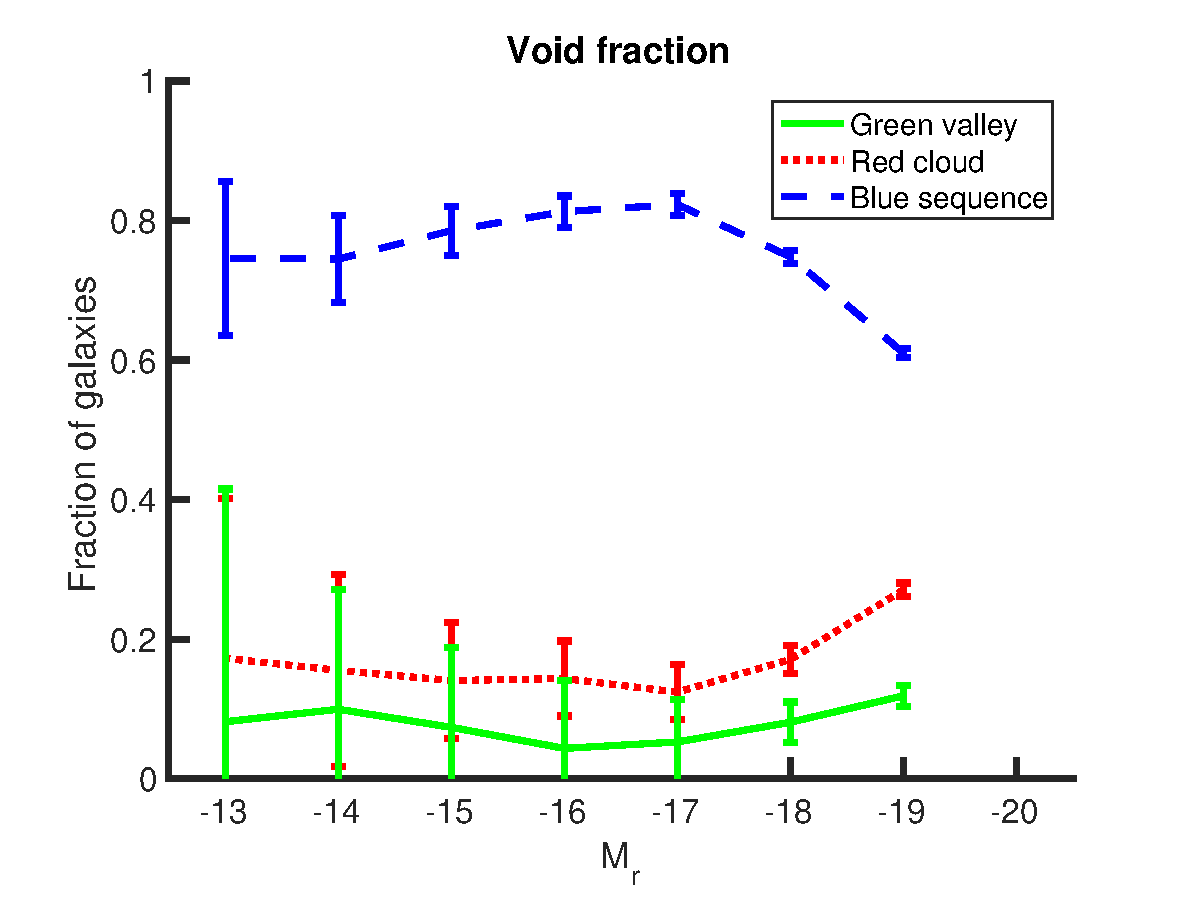
\includegraphics[width=0.49\textwidth]{Images/GV/voidFrac_CMD}
    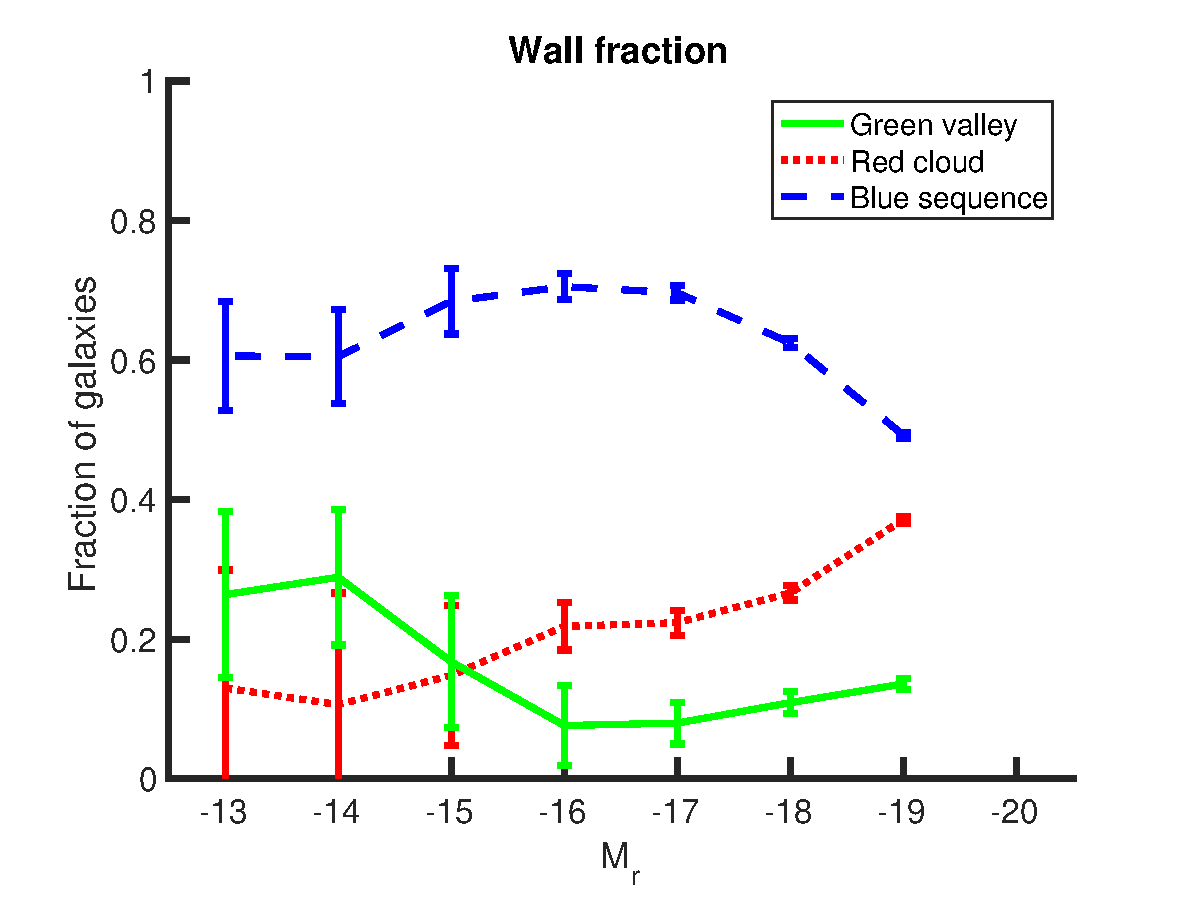
\includegraphics[width=0.49\textwidth]{Images/GV/wallFrac_CMD}
    \caption[Fraction of galaxies in CMD populations by morphological type]
    {Fraction of void (left) and wall (right) galaxies in each of the three CMD 
    populations, classified by the morphological type listed in the KIAS-VAGC.  
    There is a higher fraction of green valley dwarf galaxies ($M_r > -17$) 
    found in the more dense environments than in the voids.  This would indicate 
    that void galaxies are slightly behind wall galaxies in their evolution, 
    matching predictions based on the $\Lambda$CDM cosmology.}
    \label{fig:Mr_bin}
\end{figure}

When we separate the galaxies in each of the three populations by their 
large-scale environment, we discover a variation in these populations as a 
function of luminosity.  As we see in Fig. \ref{fig:Mr_bin}, the fraction of 
galaxies in the green valley depends on the large-scale environment, even at 
fixed stellar mass or luminosity.  A larger fraction of faint wall galaxies are 
found in the green valley than for faint void galaxies.


%%%%%%%%%%%%%%%%%%%%%%%%%%%%%%%%%%%%%%%%%%%%%%%%%%%%%%%%%%%%%%%%%%%%%%%%%%%%%%%%
%%%%%%%%%%%%%%%%%%%%%%%%%%%%%%%%%%%%%%%%%%%%%%%%%%%%%%%%%%%%%%%%%%%%%%%%%%%%%%%%


\section[Discussion]{Understanding green valley galaxies}\label{sec:discussion_GV}

Galaxies in the green valley are described to be in a transitional period of the 
galaxy's life cycle, where they are being quenched in their star formation or 
are beginning to form stars after being quiescent.  Here, we are able to 
quantitatively define galaxies in the green valley of the UV-optical CMD.  We 
find them to be of comparable stellar mass to galaxies in the red cloud, have 
intermediate SFRs and intermediate-to-low sSFRs, and have higher gas-phase 
nitrogen abundances and N/O ratios than galaxies in the blue sequence.

The range of stellar masses in galaxies from the green valley in Fig. 
\ref{fig:M_hist} shows us that these galaxies have completed most of their star 
formation.  They have acquired enough stars to have converted much of their gas 
into heavier elements.  Combined with the intermediate SFRs and 
intermediate-to-low sSFRs seen in Fig. \ref{fig:SFR_hist}, this tells us that 
these galaxies are no longer forming stars at a high rate.  This is most likely 
due to an extinction of available cool gas from which to form stars.  These 
galaxies are reaching a natural point in their evolution where they transition 
from an active star formation period to a quieter, more quiescent lifestyle.

As explained in \cite{Douglass17b}, nitrogen is thought to be produced in both a 
primary and secondary stage, depending on the presence of other heavy elements.  
The fact that the galaxies in the green valley have higher nitrogen abundances 
compared to those in the blue sequence indicate that they are building up a 
surplus of nitrogen, most likely due to the presence of heavier elements in 
later episodes of star formation.  The surplus of heavier elements allows the 
CNO cycle to commence earlier in the stars' lifetimes, producing nitrogen at a 
higher rate than oxygen.  It is also possible that the higher nitrogen 
abundances are a sign that the galaxies' intermediate mass stars (those 
primarily responsible for nitrogen synthesis) have expired.  This surplus of 
nitrogen results in the high N/O ratios seen for the green valley galaxies in 
Fig. \ref{fig:Z_hist}.

Fig. \ref{fig:Mr_bin} shows a higher fraction of faint wall galaxies than faint 
void galaxies are in the green valley.  This would indicate that void galaxies 
are slightly behind wall galaxies in their evolution, matching predictions based 
on the $\Lambda$CDM cosmology.  These results also coincide with the 
observations of \cite{Douglass17b} and Douglass \& Vogeley (2017, in prep).  
They find that, for dwarf galaxies ($M_r > -17$), those which exist in voids may 
have commenced their star formation at a later time.  The higher fraction of 
wall dwarf galaxies in the green valley might also point to an environmental 
influence on the reason for transitioning through the green valley, such as ram 
pressure stripping, which would occur much less frequently in the void 
environment.  However, the existence of void galaxies in the green valley 
indicate that galaxy interactions cannot be the only star formation quenching 
mechanism.


\subsection{Gas content indicators}

% Are there other markers in the gas content of these galaxies? 
If a galaxy's star formation is quenched due to a loss of cold gas, then its 
H{\sc i} content will be lower than other galaxies of a similar stellar mass and 
large-scale environment.  \cite{Schawinski14} finds that 48\% of the late-type 
galaxies they define to be in the green valley have \ion{H}{1} detections in the 
ALFALFA survey, consistent with a high probability of gas resevoir retention.  
Likewise, \cite{Catinella12} shows that the gas fraction ($M_{\ion{H}{1}}/M_*$) 
correlates with the NUV$-r$ color, suggesting that the transition of galaxies 
into the green valley is not due to an abrupt change in the galaxy's neutral gas 
supply.  If it is quenched due to a high gas temperature (from AGN or supernovae 
feedback), then the temperature of the gas will be higher than others of a 
similar size.  These factors will also help to determine when and why a galaxy 
transitions from star-forming to quiescent (and maybe back to star-forming).


\subsection{Evidence of AGN feedback}

\begin{figure}
    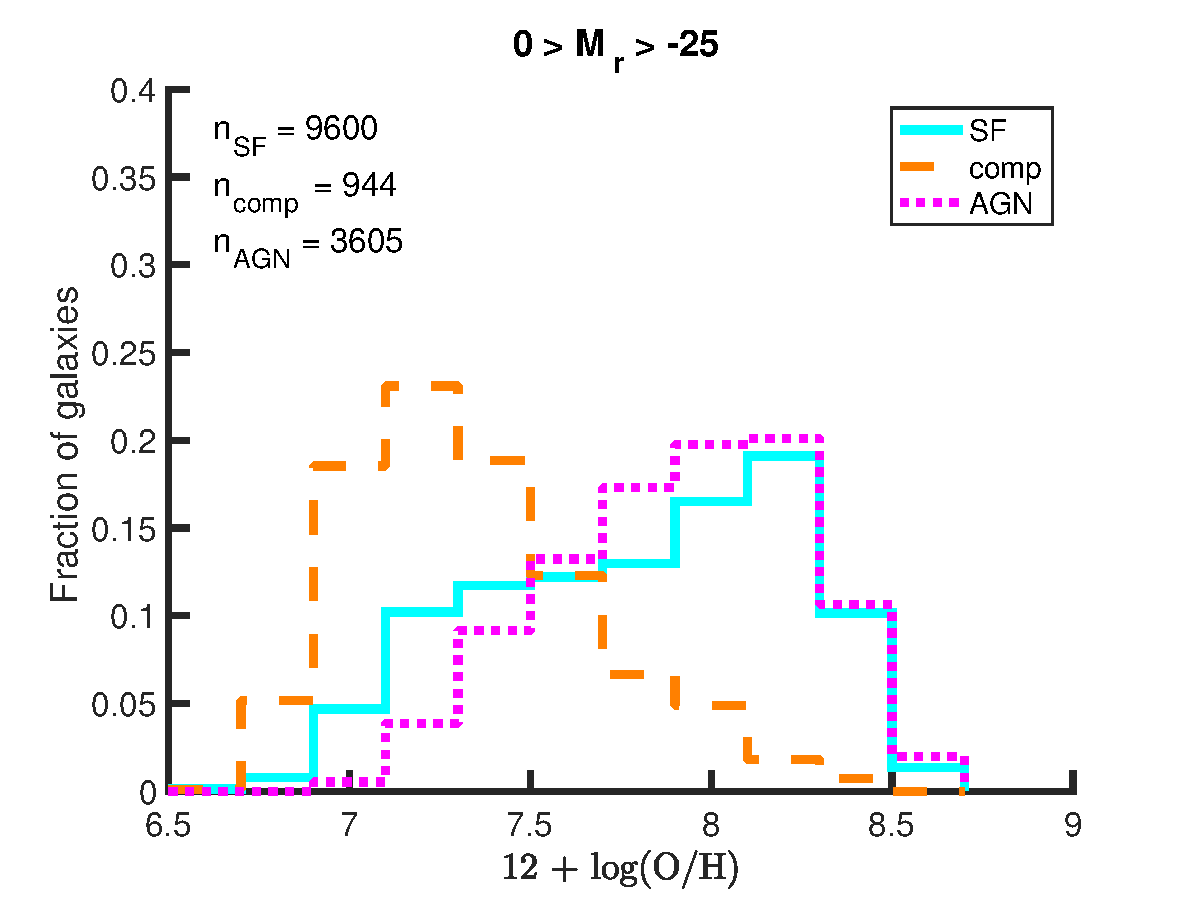
\includegraphics[width=0.49\textwidth]{Images/GV/1sig_all_BPT_t3_12logOHrelations_dust_hist}
    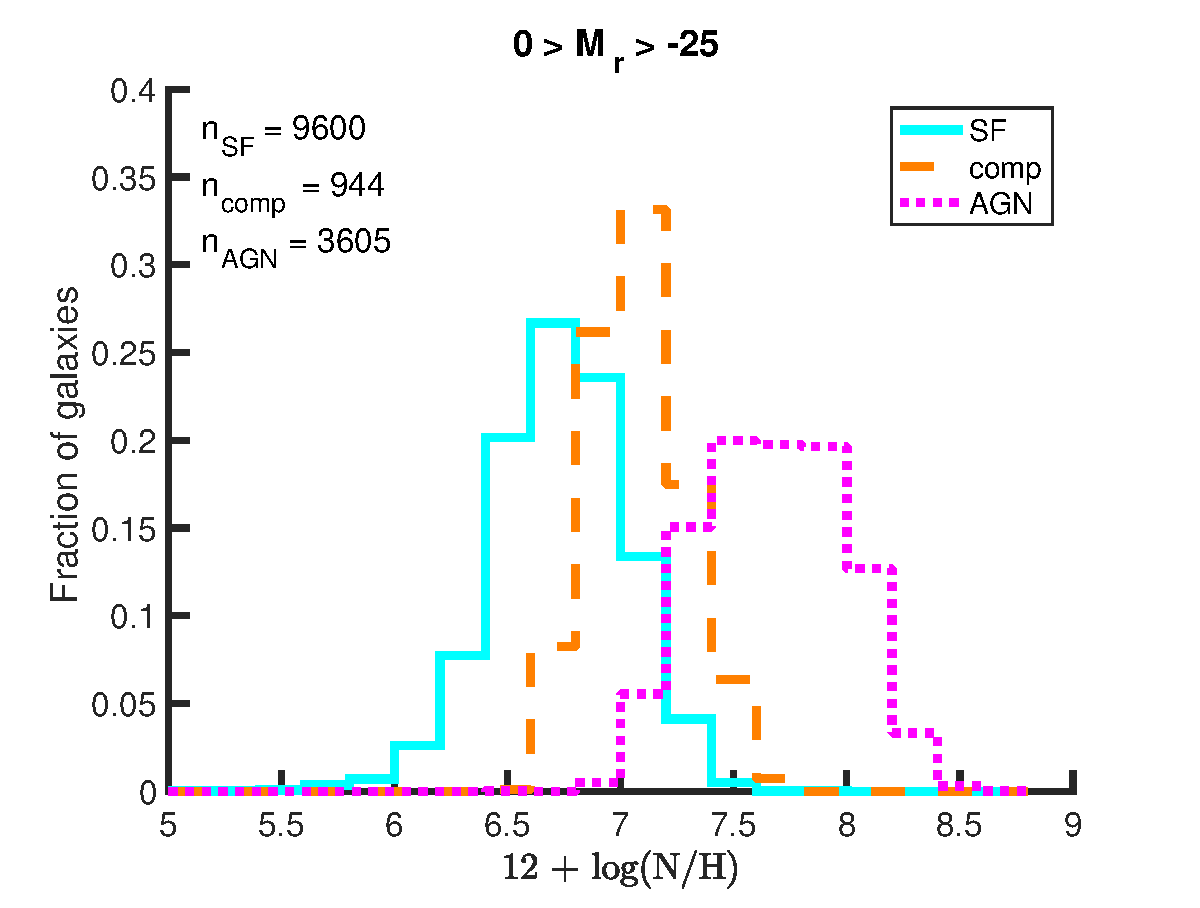
\includegraphics[width=0.49\textwidth]{Images/GV/1sig_all_BPT_t3_12logNHrelations_dust_hist}
    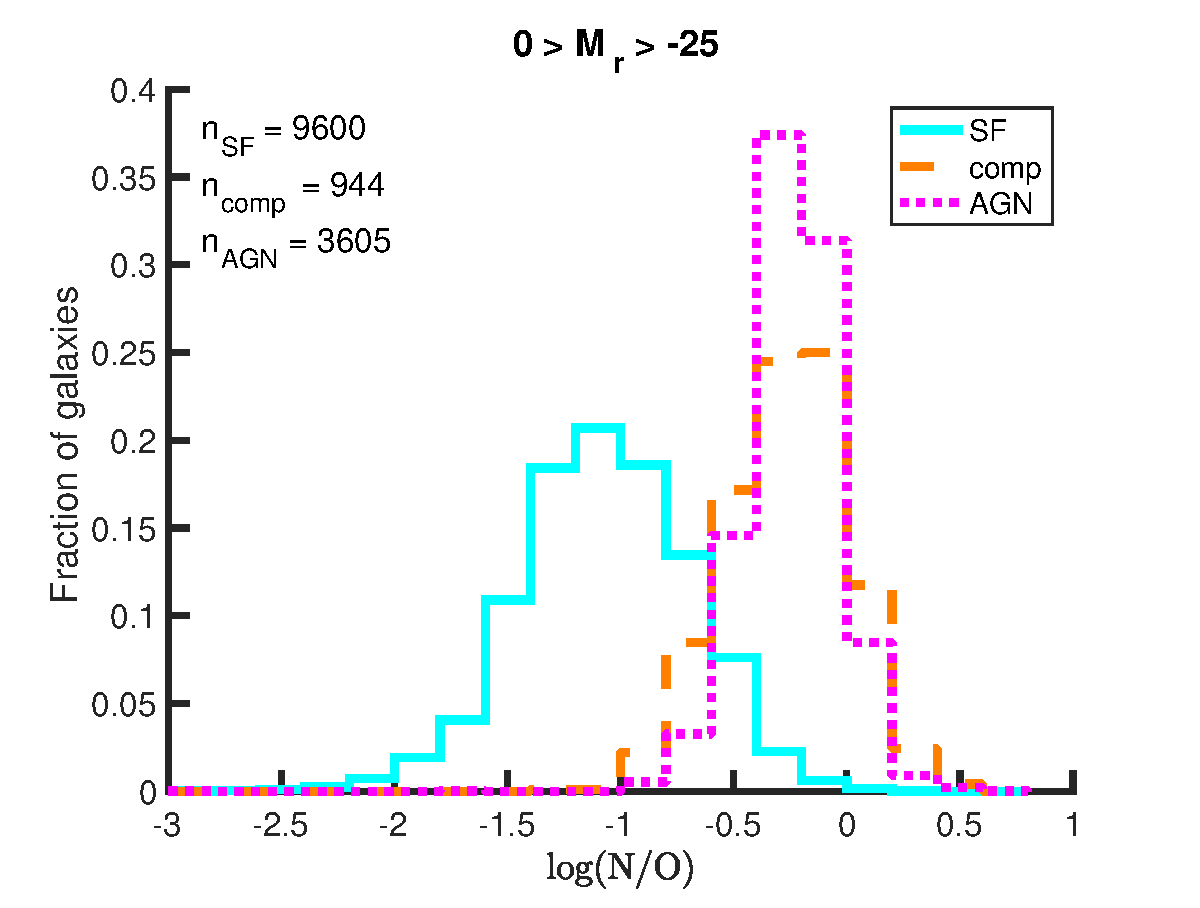
\includegraphics[width=0.49\textwidth]{Images/GV/1sig_all_BPT_t3_logNOrelations_dust_hist}
    \caption[Gas-phase chemical abundance distributions for star-forming, 
    composite, and AGN galaxies]{Distribution of the gas-phase oxygen abundance 
    (O/H, top left), nitrogen abundance (N/H, top right), and N/O ratio (bottom 
    center) of the SDSS DR7 galaxies with detectable emission lines for 
    abundance calculations with the Direct $T_e$ method.  Star-forming galaxies 
    are shown with a solid cyan line, while composite galaxies are a dashed 
    orange line and galaxies with an AGN are represented as a dotted magenta 
    line.  Composite galaxies have lower oxygen abundances than both 
    star-forming galaxies and those with an AGN.  The nitrogen abundance range 
    is different for each of the three classes, with star-forming galaxies 
    having the lowest nitrogen abundances, AGN having the highest, and 
    composite galaxies in the middle.  Therefore, star-forming galaxies have 
    N/O ratios $< 0$, while composite galaxies and galaxies with an AGN have 
    N/O ratios between -1 and 0.5.}
    \label{fig:BPT_abund}
\end{figure}

Galaxies can be classified into a number of categories with the use of a BPT 
diagram \citep{Baldwin81}.  By comparing different emission line ratios to get 
an idea of the hardness of the spectrum, we can identify if most of the energy 
in the galaxy's spectrum is coming from a star-forming region, an AGN, or a 
combination of both (``composite'').  To understand the gas-phase chemical 
abundances of the green valley galaxies, we compare Fig. \ref{fig:Z_hist} with 
the distribution of the gas-phase chemical abundances of star-forming and 
composite galaxies and galaxies with an AGN shown in Fig. \ref{fig:BPT_abund}; 
the BPT diagram classifications are from \cite{Brinchmann04}.  We see that the 
galaxies with an AGN have the most similar distributions in the three abundance 
ratios as the green valley galaxies: both groups have similar oxygen abundances 
(O/H) and higher nitrogen abundances (N/H) and N/O ratios than the star-forming 
galaxies.  This might indicate a link between green valley galaxies and a host 
AGN.  The presence of an AGN in green valley galaxies would support other 
studies of the transition of galaxies from the blue sequence to the red cloud, 
which attribute the quenching of star formation to accretion of a central black 
hole \citep[e.g.,][]{Croton06,Stasinska08}.



%%%%%%%%%%%%%%%%%%%%%%%%%%%%%%%%%%%%%%%%%%%%%%%%%%%%%%%%%%%%%%%%%%%%%%%%%%%%%%%%
%%%%%%%%%%%%%%%%%%%%%%%%%%%%%%%%%%%%%%%%%%%%%%%%%%%%%%%%%%%%%%%%%%%%%%%%%%%%%%%%


\section[Conclusions]{Conclusions}

We find a remarkable conformity between galaxies identified by morphological 
classification and their location in the NUV$-r$ CMD, which clearly identifies 
the green valley.  We can define galaxies which are transitioning through the 
green valley of the color-magnitude diagram by combining the galaxy's color, 
color gradient, and inverse concentration index.  Using these properties for the 
morphological classification, galaxies with a value less than 25 for the 
morphological type as calculated in the KIAS-VAGC exist in the green valley 
portion of the UV-optical color magnitude diagram.  Galaxies defined as early 
types (morphological type values equal to 1 or 2) are in the red cloud, while 
those with morphological type values greater than 25 are in the blue sequence.  
With this quantitative definition for galaxies transitioning through the green 
valley, we can begin to understand the properties of green valley galaxies and 
the evolution of galaxies.

Based on our analysis, green valley galaxies have stellar masses comparable to 
those in the red cloud.  They have intermediate SFRs, and low-to-intermediate 
sSFRs.  Green valley galaxies also have high gas-phase nitrogen abundances (N/H), 
resulting in high N/O ratios.  While their SFRs show that something has quenched 
their star formation, their stellar masses inform us that this is not due to any 
premature quenching mechanism.  The high nitrogen abundances in the green valley 
galaxies indicate that the galaxies are either no longer forming stars (since 
nitrogen is produced in lower mass stars than oxygen), or that the galaxies were 
able to produce both primary and secondary nitrogen (heavy elements were present 
during the last few star formation episodes to permit the CNO cycle to commence 
earlier).  This chemical abundance pattern (normal oxygen, high nitrogen, and 
high N/O ratio) is also seen in galaxies classified as AGN, indicating that the 
galaxies in the green valley have an AGN.

There is a higher fraction of faint wall galaxies than faint void galaxies in 
the green valley.  In conjunction with the conclusions of \cite{Douglass17b} and 
Douglass et al. (2017, in prep), this indicates that void dwarf galaxies are 
less evolved than dwarf galaxies in denser environments.  It would be beneficial 
to investigate the small-scale ($\sim$1 \hMpc) environment of galaxies in the 
green valley, to determine if any interactions are responsible for the 
transitional state.